\chap{Conclusion}

\section{Summary}

This study was mainly focused on having an initial approach with Data Science field, in order to investigate and document possible methods and techniques. At the same time, an another target of this work was to evaluate the feasibility of Python in Data Science, describing implementation procedures and reporting observations. \\
Specifically, this procedure was applied for reporting the initial analysis, displaying and forecasting results about Norwegian salmon farming, in order to provide structured, described and accessible data.

This study concludes showing that it's actually possible to use Python within the Data Science field. In particular, the results of this work show Python potential in this area reporting documented implementation and evidences about it, together with the main modules and packages that are describing techniques for analysis, displaying and forecasting of values.\\ 
The procedure realized during this work provides also a general idea about forecasting systems, showing the main problems and challenges, reporting possible methods that can be used for solve it or to improve it. 
Last but not least, this thesis introduces some discussion points, particularly about Evaluation system improvements [\ref{Discussion1}] and Feed consumption predictions [\ref{Discussion2}], that are providing some useful suggestions and ideas for further works in the next section [\ref{Recommendations}].

\newpage
\section{Recommendations to future work}
\label{Recommendations}
\vspace{-5mm}
In this section are reported some ideas for future work and some extra implementation that have not been implemented during this thesis due to the time limitation. Some of them could be considered interesting for future reserach or analysis.
\begin{itemize}
\item \textbf{Improve the dataset content}\\ The data collection that has done during this thesis provides just public data about territorial statistics. Would be interesting to test the same system with data coming from single reality, like for example in this case gather data from a single locality of salmon farming and then run the system on it.
\item \textbf{Visualization of the data}\\ Also if the library used during this study allow a quite good visualization of the data, it would be useful to check out other ways to realize it, which could imply the use of Python or not. For instance, if you still want to use Python could be possible to check out other libraries, such as "Plotly Python Library"\footnote{Link to Plotly Library : \url{https://plot.ly/python/}}.
\item \textbf{System as a service}\\ Would be really interesting to investigate about a possible way to provide this kind of analysis, displaying and forecasting systems like a service, such as this following simple idea:\\

\begin{figure}[H]
	\centering
       \makebox[1\textwidth][c]{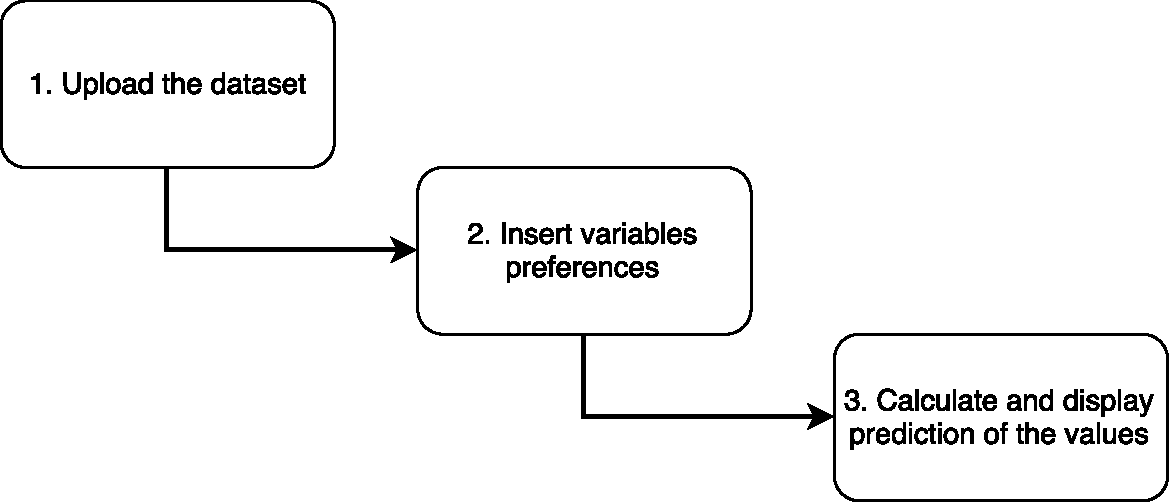
\includegraphics[width=0.8\textwidth]{Files/ServiceSystem.pdf}}
    \caption{General idea about Prediction Systems as a service.}
\end{figure}

\newpage

\item \textbf{Improve the ARIMA evaluation system}\\ Since the Evaluation system implemented during system was a very basic and easy implementation, I strongly recommend to check out the "Box–Jenkins method"\cite{wiki:BoxJenkinsMethod}. In time series analysis this method applies autoregressive integrated moving average (ARIMA) models to find the best fit of a time-series model to past values of a time series. It provide a three phase approach, that are model identification, parameter estimation and model checking. In particular, it provides a clear description of how to interpret the graphic, such as the autocorrelation plot of a series, that is very important for identify stationarity and seasonality of a series, which are indispensable details to consider if you want to improve the prediction system.

\item \textbf{Improve the prediction system}\\ This is the part which has much more possible future works. Forecasting system development is today a fundamental issue that involves different area of studies. To achieve an accurate model and significant results it needs much more specific research than the one reported in this study, that was just for report a general idea about it. I strongly recommend for further works:
\begin{itemize}
\item Improve this forecasting model, applying and studying the "Box-Jenkins method"\footnote{Box-Jenkins method : \url{https://en.wikipedia.org/wiki/Box\%E2\%80\%93Jenkins\_method}} in order to improve the Evaluation system and get better predictions of future value.z
\item If you are interested in "salmon feed consumption" forecasting I strongly suggest you to consider the discussion about the relation between "Feed Consumption" and "Average Sea Temperature", since it could provides a significant help in order to improve the accuracy level of the system.
\end{itemize}
\end{itemize}




